\documentclass{article}
\usepackage[utf8]{inputenc}
\usepackage{amsmath}
\usepackage{amsfonts}
\usepackage{amssymb}
\usepackage{graphicx}
\usepackage{geometry}
\usepackage{xcolor}
\usepackage{gensymb}
\usepackage{hyperref}
\usepackage{gensymb}
\usepackage{listings}

\newcommand{\inv}{^{-1}}   
\newcommand{\Z}{\mathbb Z}
\newcommand{\R}{\mathbb R}
\newcommand{\Q}{\mathbb Q}
\newcommand{\C}{\mathbb C}
\newcommand{\N}{\mathbb N}

\begin{document}

\newpage\noindent\textbf{1.}
\begin{center}
    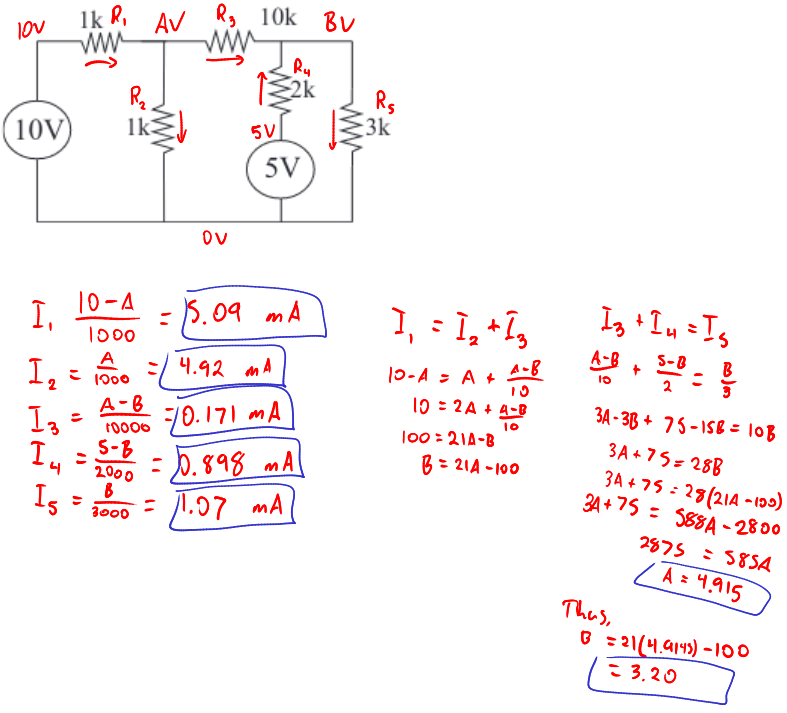
\includegraphics[scale=.7]{1.png}
\end{center}

\newpage\noindent\textbf{2.}
\begin{center}
    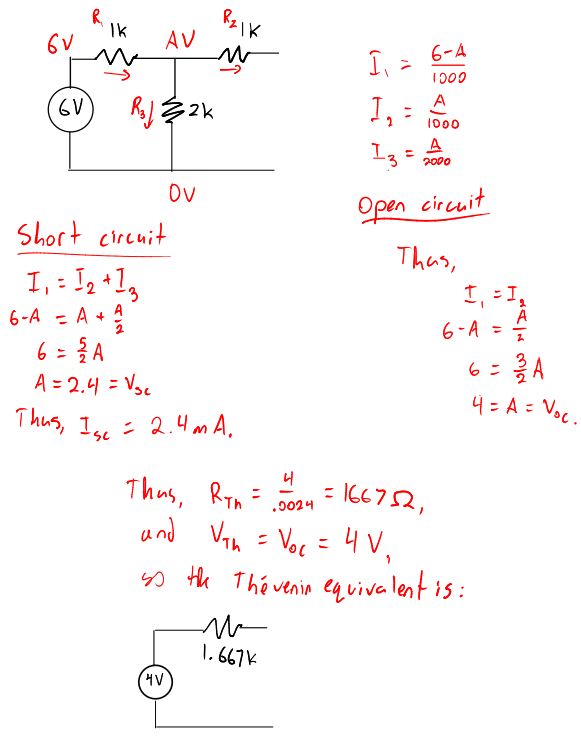
\includegraphics[scale=.7]{2.png}
\end{center}

\newpage\noindent\textbf{3.}

    When discharging begins, there is a high charge density on the negatively charged plate of the capacitor.
    Because of this, the repulsive force between electrons is high.
    As the magnitude of the charge on the plate decreases, the remaining electrons' collective repulsive force decreases, so the rate at which electrons leave the plate slows.

\newpage\noindent\textbf{4.}

    When the resistance of the variable resistor is high, then the voltage drop across it is large, so the output volume is low.
    Similarly, when the resistance is low, the voltage drop is small, so the output volume is high.
    The reason this works is that resistors provide a linear resistance, so the output wave is not distorted.

\newpage\noindent\textbf{5.}

    When 1.25A of current is drawn from the battery, there will be a $1.25 \cdot 0.4 = 0.5$V drop due to the internal resistance. Thus, in order to keep the battery terminal voltage above 1V, the current drawn must be less than 1.25A.

\newpage\noindent\textbf{6.}

    The current through the circuit is $\frac{1.5}{R + 0.4}$A.
    Thus, the power delivered to a load of resistance $R$ is $\left(\frac{1.5}{R+0.4}\right)^2R$.
    Maximizing this expression, we find that the most power is drawn when $R=0.4\Omega$.
    This amounts to 1.406W.

\newpage\noindent\textbf{7.}

    Because each flip-flop's output is connected to the next flip-flop's input, each clock cycle should shift the outputs down by one place.
    This device is called a shift register.
    Thus, after 4 clock cycles, the output will be 01101011.
    
\newpage\noindent\textbf{8.}
\begin{center}
    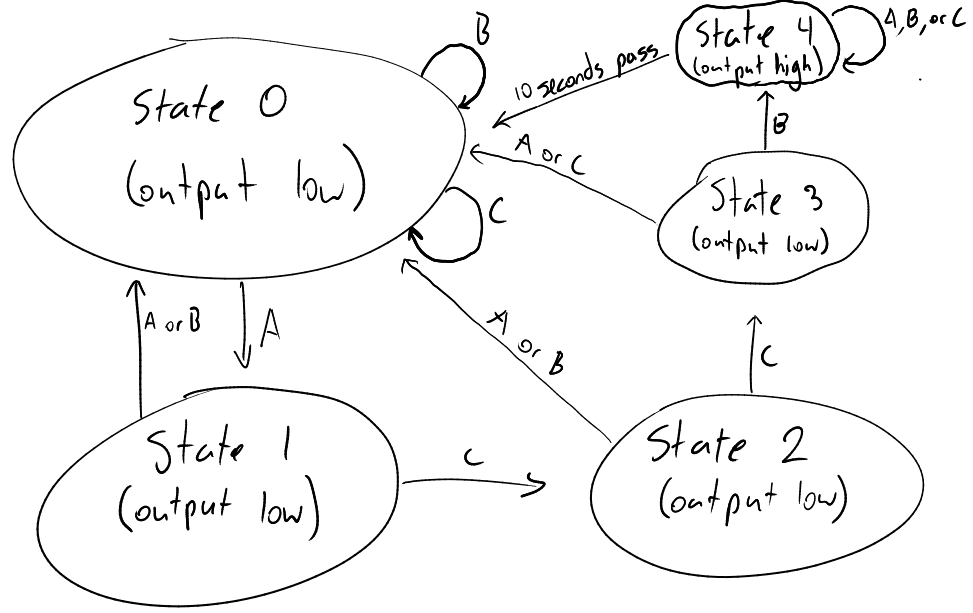
\includegraphics[scale=.6]{3.png}
\end{center}

\newpage\noindent\textbf{9.}

\newpage\noindent\textbf{10.}


\end{document}
